\documentclass[conference]{IEEEtran}
\IEEEoverridecommandlockouts
% The preceding line is only needed to identify funding in the first footnote. If that is unneeded, please comment it out.
\usepackage{cite}
\usepackage{amsmath,amssymb,amsfonts}
\usepackage{algorithmic}
\usepackage{graphicx}
\usepackage{textcomp}
\usepackage{xcolor}
\usepackage{acronym}
\usepackage{hyperref}
\usepackage{cleveref}

\acrodef{API}{Application Programming Interface}
\acrodef{AR}{Augmented Reality}
\acrodef{ACL}{Anti-Corruption Layer}
\acrodef{CLI}{Command Line Interface}
\acrodef{HCI}{Human-Computer Interaction}
\acrodef{MMI}{Man Machine Interaction}
\acrodef{HMI}{Human-Machine Interface}
\acrodef{IDE}{Integrated Development Environment}
\acrodef{LLM}{Large Language Model}
\acrodef{GUI}{Graphical User Interface}
\acrodef{UI}{User Interface}
\acrodef{YAML}{YAML Ain't Markup Language}
\acrodef{UX}{User Experience}

\def\BibTeX{{\rm B\kern-.05em{\sc i\kern-.025em b}\kern-.08em
    T\kern-.1667em\lower.7ex\hbox{E}\kern-.125emX}}
\begin{document}

\title{Enhancing Human-Computer Interaction with LLMs in Distributed Simulations\\
%\thanks{Identify applicable funding agency here. If none, delete this.}
}

\author{\IEEEauthorblockN{Angelo Filaseta}
\IEEEauthorblockA{\textit{Department of Computer Science and Engineering} \\
\textit{Alma Mater Studiorum---Università di Bologna}\\
Cesena, Italy \\
0009-0004-6797-6814}
}

\maketitle

\begin{abstract}
    Designing effective and user-friendly \acp{HMI} for simulators can be a complex endeavor that requires adherence to guidelines
    established through decades of research.
    The inherent complexity of the systems under examination contributes to the difficulty of creating intuitive interfaces that suit the user's needs.
    %
    \acp{HCI} can be particularly complex for general-purpose simulators,
    since the elements to observe and interact with can drastically change depending on the context.
    %
    Some additional challenges arise when dealing with distributed simulations,
    as the observer might want to interact with multiple simulations at once.
    %
    In this paper,
    we will explore the challenges of designing innovative \acp{HMI} for distributed general-purpose simulations,
    trying to address the issues caused by the inevitable complexity portrayed by the system.
    %
    Moreover,
    we will also discuss the potential benefits and drawbacks of using \acp{LLM} to assist the user in interacting with simulations.
\end{abstract}

%\begin{IEEEkeywords}
%    human computer interaction, distributed simulation
%\end{IEEEkeywords}

\subsection{Introduction}
\ac{HCI},
also sometimes referred to as \ac{MMI},
focus on the design, evaluation, and realization of \emph{interactive} computing systems for human use.
The effectiveness of an \ac{HMI} heavenly depends on factors that consider both \emph{usability} and \emph{functionality}~\cite{Sinha2010}.
%
The two aspects must be balanced to create easy-to-use interfaces
while providing all the necessary tools for users to reach their goals.
%
The development of interactive interface design has rapidly progressed over the past decades,
significantly focusing on the enhancement of \acp{GUI}~\cite{Murad2019}.
%
However,
research is being conducted to explore new ways to interact with machines,
with inclusions regarding,
but not limited to,
eye-tracking,
hand gesture recognition,
and \acp{LLM}~\cite{Poole2006, Sarma2021, kapania2024imcategorizingllmproductivity}.

As a matter of fact,
observability is a key aspect of simulations,
and a graphical representation is really helpful to visualize the behavior of the system.
%
Consequently,
simulators usually provide \acp{GUI} or some sort of rendering system that allow users to visualize the simulation progress.
%
\ac{CLI} and the logs generated by the simulator are also valid alternatives for observation,
even though the \ac{UX} is not as good as the \ac{GUI}.

Moreover,
\ac{AR} has been successfully used to provide additional feedback to users,
such as tactile sensations,
making simulations feel more realistic~\cite{Jud2020}.
%
Interaction can be conducted using external hardware such as mouse, keyboard, touch screen, or controllers,
and could require sensors and actuators depending on the context of the simulation.

At the same time,
\ac{LLM}s are are emerging as a new, powerful tool to interact with machines,
assisting users in reaching their goals.
%
\acp{LLM} are becoming more and more popular in very diverse fields,
spanning from code generation,
to assistance to medical doctors~\cite{Wu2024}.
%
A the time of writing,
\acp{LLM} have also been identified as a useful tool to generate simulation scenarios~\cite{Zhang2023}.

However,
the use of \ac{LLM} in the context of simulations is still an open field,
lacking cases where \ac{LLM} are used to assist users in the whole process of interacting with a simulation.

\subsection{The Alchemist Simulator as a use case}
The Alchemist simulator is a general-purpose and extensible simulator that allows to model and simulate complex systems~\cite{Pianini_2013}.
%
In order to create and describe simulation environments,
users need to create configuration files.
%
Using a \ac{CLI},
it is then possible to run simulations by providing the configuration file as an input.
%
We are currently in the process of migrating from a desktop-based \ac{GUI} to a web-based \ac{GUI} in order to tackle some limitations and enhance the \ac{UX} for a number of motivations:
\begin{enumerate}
    \item \emph{usability} increases,
    since users can interact with simulations using a a web browser on any device,
    including smartphones and tablets;
    \item adding new \emph{functionalities} becomes easier,
    since there are many tools oriented to data visualization,
    such as libraries for plotting data.
\end{enumerate}
%
%The first problem can be addressed by using languages which support a variety of platforms as targets for compilation,
%to make the usage of the same data structures in different environments possible~\cite{DBLP:conf/dais/FilasetaP23}.
%
%Unfortunately, there also are some drawbacks to consider:
%\begin{enumerate}
%    \item in order to operate with the simulations component in a different ecosystem,
%    a mediation layer is needed to translates the semantic of the domain model,
%    leading  to an additional piece of code need to be implemented and maintained;
%    \item the web environment is not as performant as a native application.
%    Continuously rendering images in real-time can be really demanding.
%\end{enumerate}
%
%
%%
%%
%The performance problem is much harder to address,
%and could be mitigated by including WebAssembly in the technology stack,
%which has been proved to be more efficient and performant than the most used web language,
%JavaScript,
%in compute-intensive cases~\cite{DBLP:conf/ict4s/Macedo0PS22}.
%%
Additionally,
the web ecosystem is suitable for facilitating effective communication between multiple distributed endpoints,
also providing more support in linking external services,
such as \ac{LLM},
which are usually available as a service accessible via \acp{API}.
%
\subsection{A comparison of \ac{LLM} in \acp{IDE} and Simulations}
A software is usually an enabler for a user to reach a goal of some sort.
%
In the case of \acp{IDE}, the main goal is to create source code that,
when compiled and executed,
produces an expected result.
%
Indeed,
An IDE is an adequate tool that provide the user the functionality to write code,
but it can be enrich with additional functionalities to boost the \ac{UX} even more.
%
Nowadays,
it is common for \acp{IDE} to include tools like GitHub Copilot\footnote{
    GitHub Copilot · Your AI pair programmer, \url{http://archive.today/jsEIH}
} to further assist users in writing code.
%
Such tools can successfully be used as effective pair programming tools by experienced developers~\cite{DBLP:journals/jss/DakhelMNKDJ23}.
%

Simulations are not different from an \ac{IDE} in this regard,
as they are an enabler to visualize and observe a designed and defined representation of processes.
%
\begin{figure}
    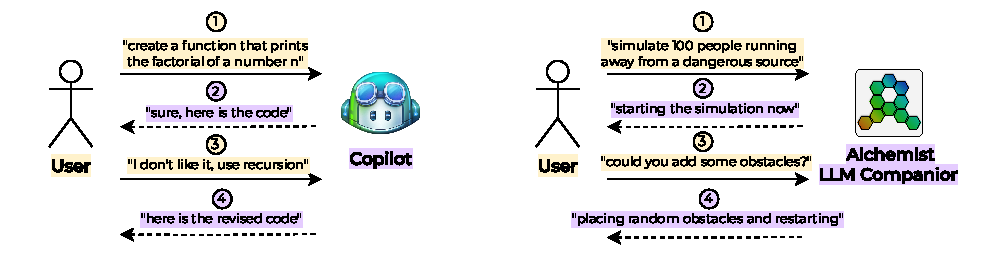
\includegraphics[width=\columnwidth]{use-case}
    \caption{
        Comparison between the usage of an LLM in code generation (left) and in a simulation (right).
        %
        The lower block represent the tool used by a user to reach the goal, represented by the upper block.
        %
        The blocks in the middle represent the additional tools based on LLM that can be used to assist the user.
    %
    }
    \label{fig:usecase}
\end{figure}
%
\Cref{fig:usecase} shows a comparison of the usage of an \ac{LLM} in code generation and in simulations.
%
Copilot is used to assist the user in writing code,
and is able to generate pieces of code that fulfill the user's needs.
%
Users can also write code by hand on their own using the \ac{IDE}'s basic functionalities,
but are not limited to it.
%
The same concept can be applied to simulations,
where an \ac{LLM} can be used to assist the user in configuring the simulator and interact with it.
%
This can be helpful since configuring Alchemist by hand can be time-consuming,
especially for new users that are not familiar with the domain model and the semantics.
%
On the other hand,
describing a simulation scenario in natural language is usually easier.
%
Ideally
there are several other use cases in which an \ac{LLM} can become really handy while interacting with a simulation, apart from generating configurations.
%
The \ac{LLM} could become a real assistant for the user,
providing multiple functionalities to assist the user in interacting with the simulation.
%

Imagine a complex scenario of a distributed simulation: a pool of network nodes is available,
and an inexperienced user wants to create a number of differently parameterized simulations,
and run one of each for each node.
%
The user would firstly need to understand the domain model,
create the configuration files,
understand how to start the engine and finally link a \ac{GUI} to visualize the simulation progress.
%
The inclusion of an \ac{LLM} would not only assist the user with problems related to the domain model,
but also enable the user to generate the required files and run the simulation in the way described,
if possible.
%

There are plenty of model and techniques available to apply \ac{LLM},
based on the specific use case.
%
One example that could suite the simulation use case is the ReAct prompting technique~\cite{DBLP:conf/iclr/YaoZYDSN023},
which focuses on generating both reasoning traces and task-specific actions.
%
Moreover,
the framework is also able to retrieve information from external environments,
enabling for avoidance of fact hallucination.
%
However,
the best way to design of an \ac{LLM} depends on a variety of factors,
and still needs research to be conducted.
% Other things about LLM... to write
\subsection{Conclusion and Future Works}
The Alchemist simulator was used as a case study,
proposing a transition from a desktop-based \ac{GUI} to a web-based \ac{GUI} to overcome some limitations and increase the amount of support that external tools can provide.
%
The inclusion of \ac{LLM} in the simulation could result very beneficial in terms of \ac{UX},
but research still needs to be conducted in order to understand how to effectively design an \ac{LLM} that can assist users in interacting with simulations.
%
\ac{LLM} and similar technologies are promising and pervasive tools that can be used to assist users in solving everyday problems,
and simulations are no exception.
%
%
There are several possible way to effectively design an \ac{LLM} in order to improve the prompts and get better results,
and we will work to find the best way to interact with the simulator.

\bibliographystyle{IEEEtran}
\bibliography{doctoral-colloquium-2024-dsrt-simulation-interaction}
\vspace{12pt}
\end{document}


